\documentclass[]{article}

\usepackage[dvipsnames]{xcolor}
\usepackage[landscape,margin=1cm]{geometry}
\usepackage{multicol}
\usepackage{graphicx}
\usepackage{amsmath}
\pagestyle{empty}
\usepackage{float}
\usepackage{physics}
\usepackage{subfiles}

\begin{document}
\begin{multicols}{3}
\section{Courbes de Bézier}
\begin{center}
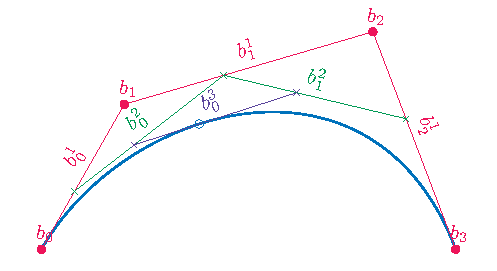
\includegraphics[width=0.6\columnwidth,page=1]{drwg_0.pdf}
\end{center}
\subsection{Triangle de Pascal}
\begin{center}
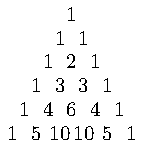
\includegraphics[scale=1,page=1]{drwg_1.pdf}
\end{center}
$$(a+b)^3=a^3+3a^2b+3ab^2+b^3$$
$$(a+b)^n=\sum_{k=0}^{n}\begin{pmatrix}
n\\k
\end{pmatrix}x^ky^{n-k}$$

$$\begin{pmatrix}
n\\ k
\end{pmatrix}=C^{n}_{k}=\frac{n!}{k!(n-k)!}$$
\subsection{Polynômes de Bernstein}
$$B_{i}^{m}(t)=\begin{pmatrix}m\\i\end{pmatrix}t^{i}(1-t)^{m-i}$$
\begin{center}
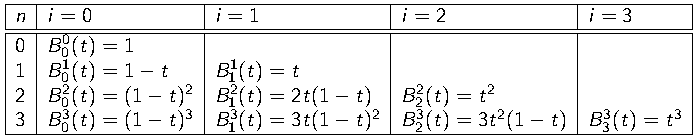
\includegraphics[width=\columnwidth]{img_21.pdf}
\end{center}
\section{Résolution numérique}
\subsection{Doolittle}
$$\begin{pmatrix}
a_{11} & a_{12} & a_{13}\\
a_{21} & a_{22} & a_{23}\\
a_{31} & a_{32} & a_{33}
\end{pmatrix}=\begin{pmatrix}
1 & 0 & 0\\
l_{21} & 1 & 0\\
l_{31} & l_{32} & 1
\end{pmatrix}\begin{pmatrix}
u_{11} & u_{12} & u_{13}\\
0 & u_{22} & u_{23}\\
0 & 0 & u_{33}
\end{pmatrix}$$
\begin{figure}[H]
\centering
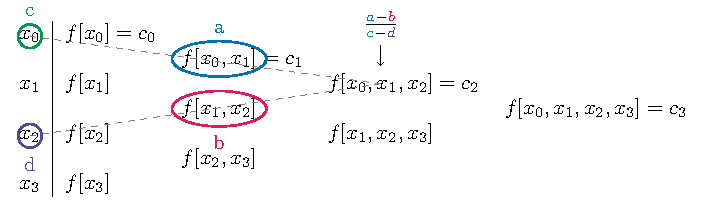
\includegraphics[scale=1,page=1]{drwg_3.pdf}
\end{figure}
\begin{align*}
(1)&\begin{cases}
u_{11}&=a_{11}\\
u_{12}&=a_{12}\\
u_{13}&=a_{13}
\end{cases} \qquad (2)\begin{cases}
l_{21}&=\frac{a_{21}}{u_{11}}\\
l_{31}&=\frac{a_{31}}{u_{11}}
\end{cases}\\
(3)&\begin{cases}
u_{22}&=a_{22}-l_{21}u_{12}\\
u_{23}&=a_{23}-l_{21}u_{13}
\end{cases} \qquad(4)\begin{cases}
l_{32}=\frac{a_{32}-l_{31}u_{12}}{u_{22}}
\end{cases}\\
(5)&\begin{cases}u_{33}=a_{33}-l_{31}u_{13}-l_{32}u_{23}\end{cases}
\end{align*}
\subsection{Cholesky}
$$\begin{pmatrix}
a_{11} & a_{12} & a_{13}\\
a_{12} & a_{22} & a_{23}\\
a_{13} & a_{23} & a_{33}
\end{pmatrix}=\begin{pmatrix}
\hat{l}_{11} & 0 & 0\\
\hat{l}_{21} & \hat{l}_{22} & 0\\
\hat{l}_{31} & \hat{l}_{32} & \tilde{l}_{33}
\end{pmatrix}\cdot\begin{pmatrix}
\hat{l}_{11} & \hat{l}_{21} & \hat{l}_{31}\\
0 & \hat{l}_{22} & \hat{l}_{32}\\
0 & 0 & \tilde{l}_{33}
\end{pmatrix}$$
\begin{align*}
\hat{l}_{11}&=\sqrt{a_{11}} & \hat{l}_{21}&=\frac{a_{12}}{\sqrt{a_{11}}}\\
\hat{l}_{31}&=\frac{a_{13}}{\sqrt{a_{11}}} & \hat{l}_{22}&=\sqrt{a_{22}-\frac{a_{12}}{\sqrt{a_{11}}}}\\
\hat{l}_{32}&=\frac{a_{23}-\frac{a_{13}a_{12}}{a_{11}}}{\sqrt{a_{22}-\frac{a_{12}}{a_{11}}}} & \hat{l}_{33}&=\sqrt{a_{33}-\hat{l}_{31}^2-\hat{l}_{32}^2}
\end{align*}
\subsection{Permutations}
Attention, si on utilise des permutations, alors
$$PA\vec{x}=P\vec{b}$$
\subsection{Méthode QR}
On commence avec une matrice $A_{n\times n}$
\begin{enumerate}
\item Prendre le premier vecteur colonne de $A$ : $\vec{v}_1$
\item Faire la décomposition pour obtenir $H_1$
\item Construire $H_1A$ puis prendre $v_2$ (première colonne de $H_1A$ \textbf{sans la première ligne et sans la première colonne}
\item à la fin, déterminer $R$ et $Q$
\end{enumerate}
$$H_nH_{n-1}\cdots H_2H_1A=R\longrightarrow A=\underbrace{H_1H_2\cdots H_{n-1}^TH_n^T}_{Q}R$$
$v$ est un vecteur de norme $1$, on utilise $\tilde{v}$ si la norme est plus grande
$$\vec{v}=\frac{\vec{n}}{\abs{\abs{\vec{n}}}}\qquad \vec{n}=x-y$$
$$y=\rho\begin{pmatrix}
1\\0\\\vdots\\0
\end{pmatrix}=\text{signe}(x_i)\abs{\abs{x_i}}\left.\begin{pmatrix}
1\\0\\\vdots\\0
\end{pmatrix}\right\rbrace\text{taille de }x$$
$$H=I-2vv^{H}$$
\subfile{resolution}
\subfile{EDO}
\section{Généralités}
\subsection{Matrices}
\subsubsection{Inverses}
$$\begin{pmatrix}
\textcolor{RoyalBlue}{a} & \textcolor{OrangeRed}{b} & \textcolor{ForestGreen}{c}\\
0 & \textcolor{Violet}{d} & \textcolor{Orange}{e}\\
0 & 0 & \textcolor{ProcessBlue}{f}
\end{pmatrix}^{-1}=\begin{pmatrix}
\frac{1}{\textcolor{RoyalBlue}{a}} & -\frac{\textcolor{OrangeRed}{b}}{\textcolor{RoyalBlue}{a}\textcolor{Violet}{d}} & \frac{\textcolor{OrangeRed}{b}\textcolor{Orange}{e}-\textcolor{ForestGreen}{c}\textcolor{Violet}{d}}{\textcolor{RoyalBlue}{a}\textcolor{Violet}{d}\textcolor{ProcessBlue}{f}}\\
0 & \frac{1}{\textcolor{Violet}{d}} & -\frac{\textcolor{Orange}{e}}{\textcolor{ProcessBlue}{f}\textcolor{Violet}{d}}\\
0 & 0 & \frac{1}{\textcolor{ProcessBlue}{f}}
\end{pmatrix}$$
Même principe si on renverse
$$\left(M^{T}\right)^{-1}=\left(M^{-1}\right)^{T}$$

$$\begin{pmatrix}
\textcolor{RoyalBlue}{a} & 0 & 0\\
\textcolor{OrangeRed}{b} & \textcolor{Violet}{d} & 0\\
\textcolor{ForestGreen}{c} & \textcolor{Orange}{e} & \textcolor{ProcessBlue}{f}
\end{pmatrix}^{-1}=\begin{pmatrix}
\frac{1}{\textcolor{RoyalBlue}{a}} & 0 & 0\\
-\frac{\textcolor{OrangeRed}{b}}{\textcolor{RoyalBlue}{a}\textcolor{Violet}{d}} & \frac{1}{\textcolor{Violet}{d}} & 0\\
\frac{\textcolor{OrangeRed}{b}\textcolor{Orange}{e}-\textcolor{ForestGreen}{c}\textcolor{Violet}{d}}{\textcolor{RoyalBlue}{a}\textcolor{Violet}{d}\textcolor{ProcessBlue}{f}} & -\frac{\textcolor{Orange}{e}}{\textcolor{ProcessBlue}{f}\textcolor{Violet}{d}} &
\frac{1}{\textcolor{ProcessBlue}{f}}
\end{pmatrix}$$
Pour une matrice $2\times 2$
$$\begin{pmatrix}
\textcolor{RoyalBlue}{a} & \textcolor{OrangeRed}{b}\\
\textcolor{ForestGreen}{c} & \textcolor{Violet}{d}
\end{pmatrix}^{-1}=\frac{1}{\textcolor{RoyalBlue}{a}\textcolor{Violet}{d}-\textcolor{OrangeRed}{b}\textcolor{ForestGreen}{c}}\begin{pmatrix}
\textcolor{Violet}{d} & \textcolor{OrangeRed}{-b}\\
\textcolor{ForestGreen}{-c} & \textcolor{RoyalBlue}{a}
\end{pmatrix}$$


\end{multicols}
\end{document}